\documentclass[twoside]{book}

% Packages required by doxygen
\usepackage{calc}
\usepackage{doxygen}
\usepackage{graphicx}
\usepackage[utf8]{inputenc}
\usepackage{makeidx}
\usepackage{multicol}
\usepackage{multirow}
\usepackage{textcomp}
\usepackage[table]{xcolor}

% Font selection
\usepackage[T1]{fontenc}
\usepackage{mathptmx}
\usepackage[scaled=.90]{helvet}
\usepackage{courier}
\usepackage{amssymb}
\usepackage{sectsty}
\renewcommand{\familydefault}{\sfdefault}
\allsectionsfont{%
  \fontseries{bc}\selectfont%
  \color{darkgray}%
}
\renewcommand{\DoxyLabelFont}{%
  \fontseries{bc}\selectfont%
  \color{darkgray}%
}

% Page & text layout
\usepackage{geometry}
\geometry{%
  a4paper,%
  top=2.5cm,%
  bottom=2.5cm,%
  left=2.5cm,%
  right=2.5cm%
}
\tolerance=750
\hfuzz=15pt
\hbadness=750
\setlength{\emergencystretch}{15pt}
\setlength{\parindent}{0cm}
\setlength{\parskip}{0.2cm}
\makeatletter
\renewcommand{\paragraph}{%
  \@startsection{paragraph}{4}{0ex}{-1.0ex}{1.0ex}{%
    \normalfont\normalsize\bfseries\SS@parafont%
  }%
}
\renewcommand{\subparagraph}{%
  \@startsection{subparagraph}{5}{0ex}{-1.0ex}{1.0ex}{%
    \normalfont\normalsize\bfseries\SS@subparafont%
  }%
}
\makeatother

% Headers & footers
\usepackage{fancyhdr}
\pagestyle{fancyplain}
\fancyhead[LE]{\fancyplain{}{\bfseries\thepage}}
\fancyhead[CE]{\fancyplain{}{}}
\fancyhead[RE]{\fancyplain{}{\bfseries\leftmark}}
\fancyhead[LO]{\fancyplain{}{\bfseries\rightmark}}
\fancyhead[CO]{\fancyplain{}{}}
\fancyhead[RO]{\fancyplain{}{\bfseries\thepage}}
\fancyfoot[LE]{\fancyplain{}{}}
\fancyfoot[CE]{\fancyplain{}{}}
\fancyfoot[RE]{\fancyplain{}{\bfseries\scriptsize Generated on Thu Nov 14 2013 11\-:57\-:06 for My Project by Doxygen }}
\fancyfoot[LO]{\fancyplain{}{\bfseries\scriptsize Generated on Thu Nov 14 2013 11\-:57\-:06 for My Project by Doxygen }}
\fancyfoot[CO]{\fancyplain{}{}}
\fancyfoot[RO]{\fancyplain{}{}}
\renewcommand{\footrulewidth}{0.4pt}
\renewcommand{\chaptermark}[1]{%
  \markboth{#1}{}%
}
\renewcommand{\sectionmark}[1]{%
  \markright{\thesection\ #1}%
}

% Indices & bibliography
\usepackage{natbib}
\usepackage[titles]{tocloft}
\setcounter{tocdepth}{3}
\setcounter{secnumdepth}{5}
\makeindex

% Hyperlinks (required, but should be loaded last)
\usepackage{ifpdf}
\ifpdf
  \usepackage[pdftex,pagebackref=true]{hyperref}
\else
  \usepackage[ps2pdf,pagebackref=true]{hyperref}
\fi
\hypersetup{%
  colorlinks=true,%
  linkcolor=blue,%
  citecolor=blue,%
  unicode%
}

% Custom commands
\newcommand{\clearemptydoublepage}{%
  \newpage{\pagestyle{empty}\cleardoublepage}%
}


%===== C O N T E N T S =====

\begin{document}

% Titlepage & ToC
\hypersetup{pageanchor=false}
\pagenumbering{roman}
\begin{titlepage}
\vspace*{7cm}
\begin{center}%
{\Large My Project }\\
\vspace*{1cm}
{\large Generated by Doxygen 1.8.5}\\
\vspace*{0.5cm}
{\small Thu Nov 14 2013 11:57:06}\\
\end{center}
\end{titlepage}
\clearemptydoublepage
\tableofcontents
\clearemptydoublepage
\pagenumbering{arabic}
\hypersetup{pageanchor=true}

%--- Begin generated contents ---
\chapter{Hierarchical Index}
\section{Class Hierarchy}
This inheritance list is sorted roughly, but not completely, alphabetically\-:\begin{DoxyCompactList}
\item Q\-Object\begin{DoxyCompactList}
\item \contentsline{section}{Penguin\-Server\-:\-:Connected\-Client}{\pageref{classPenguinServer_1_1ConnectedClient}}{}
\item \contentsline{section}{Penguin\-Server\-:\-:Shared\-List}{\pageref{classPenguinServer_1_1SharedList}}{}
\end{DoxyCompactList}
\item Q\-Tcp\-Server\begin{DoxyCompactList}
\item \contentsline{section}{Penguin\-Server\-:\-:Server\-Listener}{\pageref{classPenguinServer_1_1ServerListener}}{}
\end{DoxyCompactList}
\item Q\-Thread\begin{DoxyCompactList}
\item \contentsline{section}{Penguin\-Server\-:\-:Clients\-Manager}{\pageref{classPenguinServer_1_1ClientsManager}}{}
\item \contentsline{section}{Penguin\-Server\-:\-:Controler}{\pageref{classPenguinServer_1_1Controler}}{}
\item \contentsline{section}{Penguin\-Server\-:\-:Server\-Thread}{\pageref{classPenguinServer_1_1ServerThread}}{}
\end{DoxyCompactList}
\end{DoxyCompactList}

\chapter{Class Index}
\section{Class List}
Here are the classes, structs, unions and interfaces with brief descriptions\-:\begin{DoxyCompactList}
\item\contentsline{section}{\hyperlink{classPenguinServer_1_1ClientsManager}{Penguin\-Server\-::\-Clients\-Manager} \\*The \hyperlink{classPenguinServer_1_1ClientsManager}{Clients\-Manager} class This class represents manager of all clients. Curently this manager is responsible for resending the Clients list, but for the future will be used to manage all other issues checking state of communication and other }{\pageref{classPenguinServer_1_1ClientsManager}}{}
\item\contentsline{section}{\hyperlink{classPenguinServer_1_1ConnectedClient}{Penguin\-Server\-::\-Connected\-Client} \\*The \hyperlink{classPenguinServer_1_1ConnectedClient}{Connected\-Client} class Class represents data of client in system. Is connected to \hyperlink{classPenguinServer_1_1ServerThread}{Server\-Thread} which is operating all incomming and outcomming data }{\pageref{classPenguinServer_1_1ConnectedClient}}{}
\item\contentsline{section}{\hyperlink{classPenguinServer_1_1Controler}{Penguin\-Server\-::\-Controler} }{\pageref{classPenguinServer_1_1Controler}}{}
\item\contentsline{section}{\hyperlink{classPenguinServer_1_1ServerListener}{Penguin\-Server\-::\-Server\-Listener} \\*The \hyperlink{classPenguinServer_1_1ServerListener}{Server\-Listener} class Class represents a Tcp Listenere which manages all incomming calls }{\pageref{classPenguinServer_1_1ServerListener}}{}
\item\contentsline{section}{\hyperlink{classPenguinServer_1_1ServerThread}{Penguin\-Server\-::\-Server\-Thread} }{\pageref{classPenguinServer_1_1ServerThread}}{}
\item\contentsline{section}{\hyperlink{classPenguinServer_1_1SharedList}{Penguin\-Server\-::\-Shared\-List} \\*The \hyperlink{classPenguinServer_1_1SharedList}{Shared\-List} class }{\pageref{classPenguinServer_1_1SharedList}}{}
\end{DoxyCompactList}

\chapter{Class Documentation}
\hypertarget{classPenguinClient_1_1C2CListenThread}{\section{Penguin\-Client\-:\-:C2\-C\-Listen\-Thread Class Reference}
\label{classPenguinClient_1_1C2CListenThread}\index{Penguin\-Client\-::\-C2\-C\-Listen\-Thread@{Penguin\-Client\-::\-C2\-C\-Listen\-Thread}}
}


The \hyperlink{classPenguinClient_1_1C2CListenThread}{C2\-C\-Listen\-Thread} class class with general purpose to manage communication between clients starts T\-C\-P server, manages handshake between clients, starts U\-D\-P communication when required.  




{\ttfamily \#include $<$c2clistenthread.\-h$>$}

Inheritance diagram for Penguin\-Client\-:\-:C2\-C\-Listen\-Thread\-:\begin{figure}[H]
\begin{center}
\leavevmode
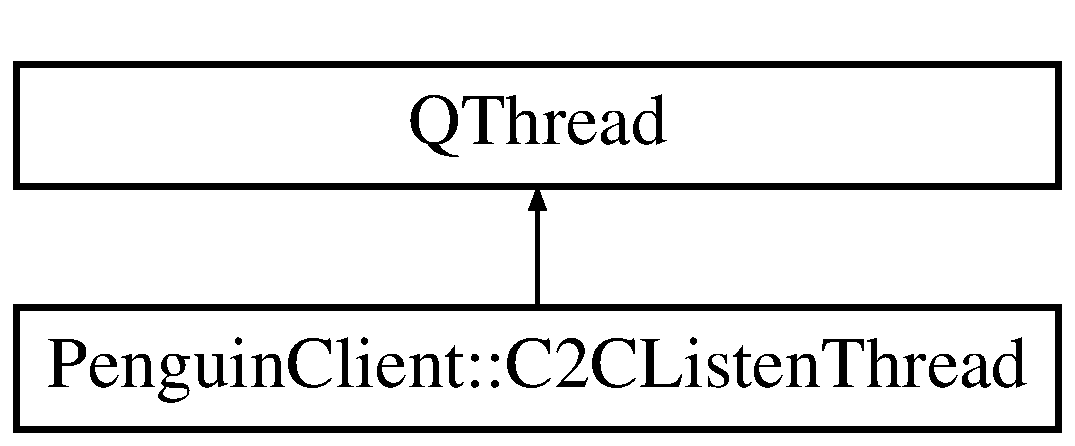
\includegraphics[height=2.000000cm]{classPenguinClient_1_1C2CListenThread}
\end{center}
\end{figure}
\subsection*{Public Slots}
\begin{DoxyCompactItemize}
\item 
\hypertarget{classPenguinClient_1_1C2CListenThread_a38a97a242e5915c5c6c22bcf04ef964c}{void {\bfseries end\-Connection} ()}\label{classPenguinClient_1_1C2CListenThread_a38a97a242e5915c5c6c22bcf04ef964c}

\end{DoxyCompactItemize}
\subsection*{Signals}
\begin{DoxyCompactItemize}
\item 
\hypertarget{classPenguinClient_1_1C2CListenThread_aad8292f0535d5fe879fb1120337dc91f}{void {\bfseries error} (int socket\-Error, const Q\-String \&message)}\label{classPenguinClient_1_1C2CListenThread_aad8292f0535d5fe879fb1120337dc91f}

\end{DoxyCompactItemize}
\subsection*{Public Member Functions}
\begin{DoxyCompactItemize}
\item 
\hypertarget{classPenguinClient_1_1C2CListenThread_a2c81ce5a877bc4709c757fb66a238695}{{\bfseries C2\-C\-Listen\-Thread} (Q\-Object $\ast$parent=0)}\label{classPenguinClient_1_1C2CListenThread_a2c81ce5a877bc4709c757fb66a238695}

\item 
void \hyperlink{classPenguinClient_1_1C2CListenThread_a3a68c0a5b439d9807805e3cac6d5a0d1}{start\-Listener} (const Q\-Host\-Address \&host\-Name, const quint16 port)
\begin{DoxyCompactList}\small\item\em start\-Listener starts this thread with given parameters \end{DoxyCompactList}\item 
\hypertarget{classPenguinClient_1_1C2CListenThread_a245f2c7a87431c92dab777dd5719836e}{void {\bfseries run} ()}\label{classPenguinClient_1_1C2CListenThread_a245f2c7a87431c92dab777dd5719836e}

\end{DoxyCompactItemize}


\subsection{Detailed Description}
The \hyperlink{classPenguinClient_1_1C2CListenThread}{C2\-C\-Listen\-Thread} class class with general purpose to manage communication between clients starts T\-C\-P server, manages handshake between clients, starts U\-D\-P communication when required. 

\subsection{Member Function Documentation}
\hypertarget{classPenguinClient_1_1C2CListenThread_a3a68c0a5b439d9807805e3cac6d5a0d1}{\index{Penguin\-Client\-::\-C2\-C\-Listen\-Thread@{Penguin\-Client\-::\-C2\-C\-Listen\-Thread}!start\-Listener@{start\-Listener}}
\index{start\-Listener@{start\-Listener}!PenguinClient::C2CListenThread@{Penguin\-Client\-::\-C2\-C\-Listen\-Thread}}
\subsubsection[{start\-Listener}]{\setlength{\rightskip}{0pt plus 5cm}void Penguin\-Client\-::\-C2\-C\-Listen\-Thread\-::start\-Listener (
\begin{DoxyParamCaption}
\item[{const Q\-Host\-Address \&}]{host\-Name, }
\item[{const quint16}]{port}
\end{DoxyParamCaption}
)}}\label{classPenguinClient_1_1C2CListenThread_a3a68c0a5b439d9807805e3cac6d5a0d1}


start\-Listener starts this thread with given parameters 


\begin{DoxyParams}{Parameters}
{\em host\-Name} & \\
\hline
{\em port} & \\
\hline
\end{DoxyParams}


The documentation for this class was generated from the following files\-:\begin{DoxyCompactItemize}
\item 
c2clistenthread.\-h\item 
c2clistenthread.\-cpp\end{DoxyCompactItemize}

\hypertarget{classPenguinClient_1_1C2CTcpListen}{\section{Penguin\-Client\-:\-:C2\-C\-Tcp\-Listen Class Reference}
\label{classPenguinClient_1_1C2CTcpListen}\index{Penguin\-Client\-::\-C2\-C\-Tcp\-Listen@{Penguin\-Client\-::\-C2\-C\-Tcp\-Listen}}
}


The \hyperlink{classPenguinClient_1_1C2CTcpListen}{C2\-C\-Tcp\-Listen} class used for management of T\-C\-P connection between clients for every new connection new thread is created.  




{\ttfamily \#include $<$c2ctcp.\-h$>$}

Inheritance diagram for Penguin\-Client\-:\-:C2\-C\-Tcp\-Listen\-:\begin{figure}[H]
\begin{center}
\leavevmode
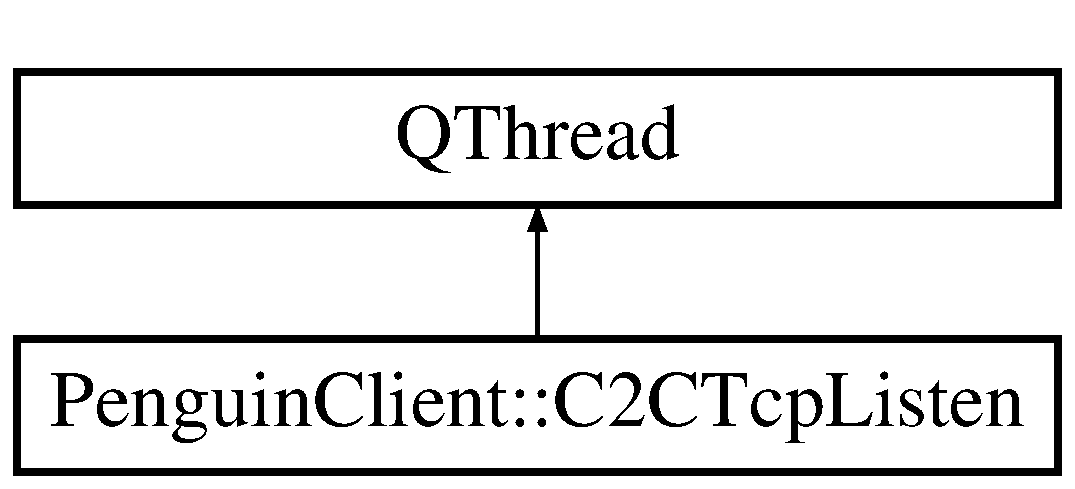
\includegraphics[height=2.000000cm]{classPenguinClient_1_1C2CTcpListen}
\end{center}
\end{figure}
\subsection*{Public Slots}
\begin{DoxyCompactItemize}
\item 
\hypertarget{classPenguinClient_1_1C2CTcpListen_ab2d0c106375767a5a3722216506000cb}{void {\bfseries ready\-Read} ()}\label{classPenguinClient_1_1C2CTcpListen_ab2d0c106375767a5a3722216506000cb}

\item 
\hypertarget{classPenguinClient_1_1C2CTcpListen_a1721622aeccb6cffeac7934cfd50e3b2}{void {\bfseries disconnected} ()}\label{classPenguinClient_1_1C2CTcpListen_a1721622aeccb6cffeac7934cfd50e3b2}

\end{DoxyCompactItemize}
\subsection*{Signals}
\begin{DoxyCompactItemize}
\item 
\hypertarget{classPenguinClient_1_1C2CTcpListen_aec51d539ea546e6e8e43b960f8d801c2}{void {\bfseries error} (Q\-Tcp\-Socket\-::\-Socket\-Error socketerror)}\label{classPenguinClient_1_1C2CTcpListen_aec51d539ea546e6e8e43b960f8d801c2}

\end{DoxyCompactItemize}
\subsection*{Public Member Functions}
\begin{DoxyCompactItemize}
\item 
\hyperlink{classPenguinClient_1_1C2CTcpListen_ac15a7392153ef8ecf33b09ef6f800e42}{C2\-C\-Tcp\-Listen} (qintptr I\-D, Q\-Object $\ast$parent=0)
\begin{DoxyCompactList}\small\item\em \hyperlink{classPenguinClient_1_1C2CTcpListen}{C2\-C\-Tcp\-Listen} used for initialization, started by T\-C\-P server by signal of incoming connection. \end{DoxyCompactList}\item 
\hypertarget{classPenguinClient_1_1C2CTcpListen_a87897f09f5c7e212edf684646e89d616}{void {\bfseries run} ()}\label{classPenguinClient_1_1C2CTcpListen_a87897f09f5c7e212edf684646e89d616}

\end{DoxyCompactItemize}


\subsection{Detailed Description}
The \hyperlink{classPenguinClient_1_1C2CTcpListen}{C2\-C\-Tcp\-Listen} class used for management of T\-C\-P connection between clients for every new connection new thread is created. 

\subsection{Constructor \& Destructor Documentation}
\hypertarget{classPenguinClient_1_1C2CTcpListen_ac15a7392153ef8ecf33b09ef6f800e42}{\index{Penguin\-Client\-::\-C2\-C\-Tcp\-Listen@{Penguin\-Client\-::\-C2\-C\-Tcp\-Listen}!C2\-C\-Tcp\-Listen@{C2\-C\-Tcp\-Listen}}
\index{C2\-C\-Tcp\-Listen@{C2\-C\-Tcp\-Listen}!PenguinClient::C2CTcpListen@{Penguin\-Client\-::\-C2\-C\-Tcp\-Listen}}
\subsubsection[{C2\-C\-Tcp\-Listen}]{\setlength{\rightskip}{0pt plus 5cm}Penguin\-Client\-::\-C2\-C\-Tcp\-Listen\-::\-C2\-C\-Tcp\-Listen (
\begin{DoxyParamCaption}
\item[{qintptr}]{I\-D, }
\item[{Q\-Object $\ast$}]{parent = {\ttfamily 0}}
\end{DoxyParamCaption}
)\hspace{0.3cm}{\ttfamily [explicit]}}}\label{classPenguinClient_1_1C2CTcpListen_ac15a7392153ef8ecf33b09ef6f800e42}


\hyperlink{classPenguinClient_1_1C2CTcpListen}{C2\-C\-Tcp\-Listen} used for initialization, started by T\-C\-P server by signal of incoming connection. 


\begin{DoxyParams}{Parameters}
{\em I\-D} & socket descriptor \\
\hline
{\em parent} & \\
\hline
\end{DoxyParams}


The documentation for this class was generated from the following files\-:\begin{DoxyCompactItemize}
\item 
c2ctcp.\-h\item 
c2ctcp.\-cpp\end{DoxyCompactItemize}

\hypertarget{classPenguinClient_1_1C2CWriteThread}{\section{Penguin\-Client\-:\-:C2\-C\-Write\-Thread Class Reference}
\label{classPenguinClient_1_1C2CWriteThread}\index{Penguin\-Client\-::\-C2\-C\-Write\-Thread@{Penguin\-Client\-::\-C2\-C\-Write\-Thread}}
}


The \hyperlink{classPenguinClient_1_1C2CWriteThread}{C2\-C\-Write\-Thread} class used for management of outgouing communication between clients.  




{\ttfamily \#include $<$c2cwritethread.\-h$>$}

Inheritance diagram for Penguin\-Client\-:\-:C2\-C\-Write\-Thread\-:\begin{figure}[H]
\begin{center}
\leavevmode
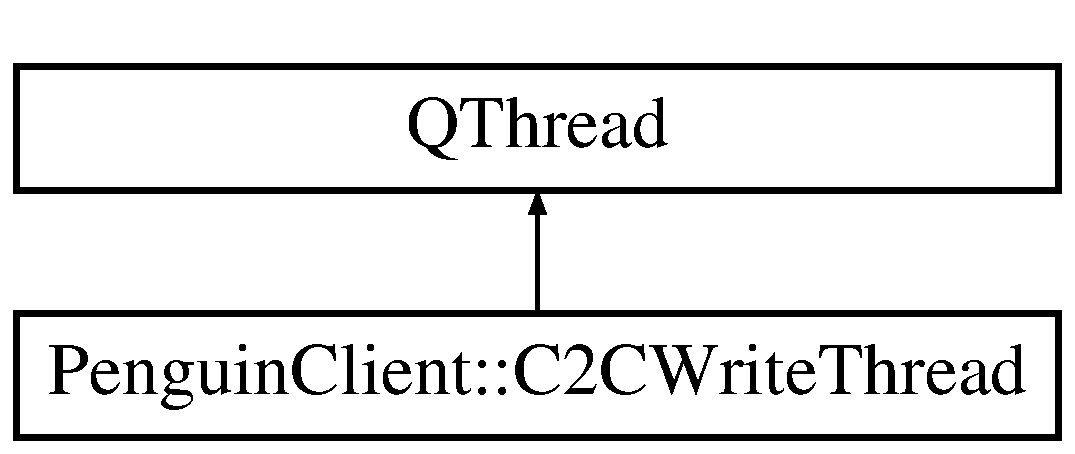
\includegraphics[height=2.000000cm]{classPenguinClient_1_1C2CWriteThread}
\end{center}
\end{figure}
\subsection*{Signals}
\begin{DoxyCompactItemize}
\item 
\hypertarget{classPenguinClient_1_1C2CWriteThread_a2c82cf0616dcd8064a1bad59d0978e3f}{void {\bfseries error} (int socket\-Error, const Q\-String \&message)}\label{classPenguinClient_1_1C2CWriteThread_a2c82cf0616dcd8064a1bad59d0978e3f}

\end{DoxyCompactItemize}
\subsection*{Public Member Functions}
\begin{DoxyCompactItemize}
\item 
\hypertarget{classPenguinClient_1_1C2CWriteThread_a9920ad27b8bf2bf9239342f0ffd5b27f}{{\bfseries C2\-C\-Write\-Thread} (Q\-Object $\ast$parent=0)}\label{classPenguinClient_1_1C2CWriteThread_a9920ad27b8bf2bf9239342f0ffd5b27f}

\item 
void \hyperlink{classPenguinClient_1_1C2CWriteThread_a69c2adce6b41b341de114bbad4cd65d6}{start\-Output} (const Q\-Host\-Address \&host\-Name, const quint16 port)
\begin{DoxyCompactList}\small\item\em start\-Output initializes thread parameters and starts thread \end{DoxyCompactList}\item 
\hypertarget{classPenguinClient_1_1C2CWriteThread_a609840686e25a73be5b85b691128705e}{void {\bfseries run} ()}\label{classPenguinClient_1_1C2CWriteThread_a609840686e25a73be5b85b691128705e}

\end{DoxyCompactItemize}


\subsection{Detailed Description}
The \hyperlink{classPenguinClient_1_1C2CWriteThread}{C2\-C\-Write\-Thread} class used for management of outgouing communication between clients. 

\subsection{Member Function Documentation}
\hypertarget{classPenguinClient_1_1C2CWriteThread_a69c2adce6b41b341de114bbad4cd65d6}{\index{Penguin\-Client\-::\-C2\-C\-Write\-Thread@{Penguin\-Client\-::\-C2\-C\-Write\-Thread}!start\-Output@{start\-Output}}
\index{start\-Output@{start\-Output}!PenguinClient::C2CWriteThread@{Penguin\-Client\-::\-C2\-C\-Write\-Thread}}
\subsubsection[{start\-Output}]{\setlength{\rightskip}{0pt plus 5cm}void Penguin\-Client\-::\-C2\-C\-Write\-Thread\-::start\-Output (
\begin{DoxyParamCaption}
\item[{const Q\-Host\-Address \&}]{host\-Name, }
\item[{const quint16}]{port}
\end{DoxyParamCaption}
)}}\label{classPenguinClient_1_1C2CWriteThread_a69c2adce6b41b341de114bbad4cd65d6}


start\-Output initializes thread parameters and starts thread 


\begin{DoxyParams}{Parameters}
{\em host\-Name} & \\
\hline
{\em port} & \\
\hline
\end{DoxyParams}


The documentation for this class was generated from the following files\-:\begin{DoxyCompactItemize}
\item 
c2cwritethread.\-h\item 
c2cwritethread.\-cpp\end{DoxyCompactItemize}

\hypertarget{classPenguinClient_1_1ClientBackgroundManager}{\section{Penguin\-Client\-:\-:Client\-Background\-Manager Class Reference}
\label{classPenguinClient_1_1ClientBackgroundManager}\index{Penguin\-Client\-::\-Client\-Background\-Manager@{Penguin\-Client\-::\-Client\-Background\-Manager}}
}
Inheritance diagram for Penguin\-Client\-:\-:Client\-Background\-Manager\-:\begin{figure}[H]
\begin{center}
\leavevmode
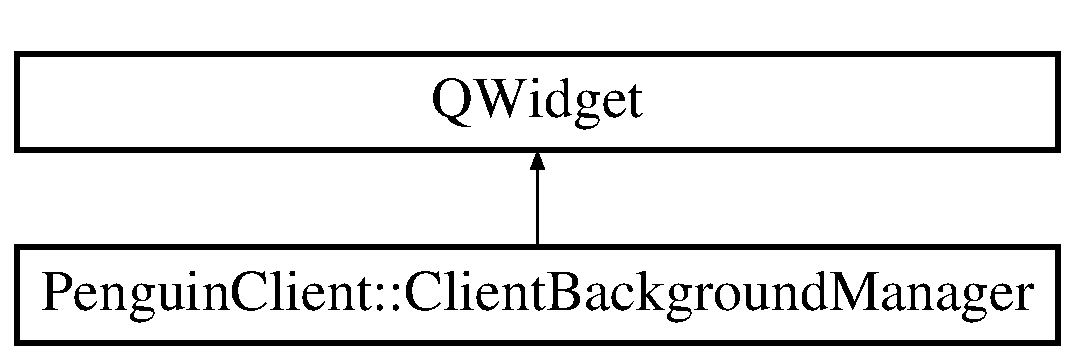
\includegraphics[height=2.000000cm]{classPenguinClient_1_1ClientBackgroundManager}
\end{center}
\end{figure}
\subsection*{Public Slots}
\begin{DoxyCompactItemize}
\item 
void \hyperlink{classPenguinClient_1_1ClientBackgroundManager_a20188400ab079c3e9007f0fa8eb3eb72}{display\-Client\-List} (const Q\-List$<$ Q\-String $>$ list)
\begin{DoxyCompactList}\small\item\em display\-Client\-List shows list of \hyperlink{classPenguinClient_1_1ClientServerThread}{Client\-Server\-Thread} \end{DoxyCompactList}\item 
void \hyperlink{classPenguinClient_1_1ClientBackgroundManager_a906fafa8aa934bd6b42eb6389cb1b13c}{incomming\-Call} (const Q\-String name, const Q\-Host\-Address I\-P, const quint16 his\-Port, const quint16 my\-Port)
\begin{DoxyCompactList}\small\item\em incomming\-Call 1. part of initialazing communication between 2 clients \end{DoxyCompactList}\item 
void \hyperlink{classPenguinClient_1_1ClientBackgroundManager_a5e403150552041e610e59c8a21f436cc}{success\-Response\-Call} (const Q\-String name, const Q\-Host\-Address I\-P, const quint16 his\-Port, const quint16 my\-Port)
\begin{DoxyCompactList}\small\item\em success\-Response\-Call 2. part of initialazing communication between 2 clients \end{DoxyCompactList}\item 
\hypertarget{classPenguinClient_1_1ClientBackgroundManager_a14b9cf4e8330646b04d9cc20c3c8266b}{void \hyperlink{classPenguinClient_1_1ClientBackgroundManager_a14b9cf4e8330646b04d9cc20c3c8266b}{incoming\-End\-Of\-Call} ()}\label{classPenguinClient_1_1ClientBackgroundManager_a14b9cf4e8330646b04d9cc20c3c8266b}

\begin{DoxyCompactList}\small\item\em incoming\-End\-Of\-Call call ended, I terminate threads between clients \end{DoxyCompactList}\item 
void \hyperlink{classPenguinClient_1_1ClientBackgroundManager_a60a97bd6e105887a188ca99d69996e48}{display\-Error} (int socket\-Error, const Q\-String \&message)
\begin{DoxyCompactList}\small\item\em display\-Error print error of Tcp\-Socket message \end{DoxyCompactList}\end{DoxyCompactItemize}
\subsection*{Signals}
\begin{DoxyCompactItemize}
\item 
\hypertarget{classPenguinClient_1_1ClientBackgroundManager_abf7ff4d2782997a9947fc191709b353e}{void {\bfseries send\-Data\-To\-Server} (Message\-Envelop \&data)}\label{classPenguinClient_1_1ClientBackgroundManager_abf7ff4d2782997a9947fc191709b353e}

\end{DoxyCompactItemize}
\subsection*{Public Member Functions}
\begin{DoxyCompactItemize}
\item 
\hypertarget{classPenguinClient_1_1ClientBackgroundManager_a93db4d3ba8a0cf57d99d2d22bc608536}{{\bfseries Client\-Background\-Manager} (Q\-Widget $\ast$parent=0)}\label{classPenguinClient_1_1ClientBackgroundManager_a93db4d3ba8a0cf57d99d2d22bc608536}

\end{DoxyCompactItemize}


\subsection{Member Function Documentation}
\hypertarget{classPenguinClient_1_1ClientBackgroundManager_a20188400ab079c3e9007f0fa8eb3eb72}{\index{Penguin\-Client\-::\-Client\-Background\-Manager@{Penguin\-Client\-::\-Client\-Background\-Manager}!display\-Client\-List@{display\-Client\-List}}
\index{display\-Client\-List@{display\-Client\-List}!PenguinClient::ClientBackgroundManager@{Penguin\-Client\-::\-Client\-Background\-Manager}}
\subsubsection[{display\-Client\-List}]{\setlength{\rightskip}{0pt plus 5cm}void Penguin\-Client\-::\-Client\-Background\-Manager\-::display\-Client\-List (
\begin{DoxyParamCaption}
\item[{const Q\-List$<$ Q\-String $>$}]{list}
\end{DoxyParamCaption}
)\hspace{0.3cm}{\ttfamily [slot]}}}\label{classPenguinClient_1_1ClientBackgroundManager_a20188400ab079c3e9007f0fa8eb3eb72}


display\-Client\-List shows list of \hyperlink{classPenguinClient_1_1ClientServerThread}{Client\-Server\-Thread} 


\begin{DoxyParams}[1]{Parameters}
\mbox{\tt in}  & {\em list} & Q\-List$<$\-Q\-String$>$ of clients logins actually are dymamical generated buttons inactive client list is printed by q\-Debug(), static buttons just for 2 clients \\
\hline
\end{DoxyParams}
\hypertarget{classPenguinClient_1_1ClientBackgroundManager_a60a97bd6e105887a188ca99d69996e48}{\index{Penguin\-Client\-::\-Client\-Background\-Manager@{Penguin\-Client\-::\-Client\-Background\-Manager}!display\-Error@{display\-Error}}
\index{display\-Error@{display\-Error}!PenguinClient::ClientBackgroundManager@{Penguin\-Client\-::\-Client\-Background\-Manager}}
\subsubsection[{display\-Error}]{\setlength{\rightskip}{0pt plus 5cm}void Penguin\-Client\-::\-Client\-Background\-Manager\-::display\-Error (
\begin{DoxyParamCaption}
\item[{int}]{socket\-Error, }
\item[{const Q\-String \&}]{message}
\end{DoxyParamCaption}
)\hspace{0.3cm}{\ttfamily [slot]}}}\label{classPenguinClient_1_1ClientBackgroundManager_a60a97bd6e105887a188ca99d69996e48}


display\-Error print error of Tcp\-Socket message 


\begin{DoxyParams}{Parameters}
{\em socket\-Error} & number of error \\
\hline
{\em message} & string version error external signal is used, call internal method \\
\hline
\end{DoxyParams}
\hypertarget{classPenguinClient_1_1ClientBackgroundManager_a906fafa8aa934bd6b42eb6389cb1b13c}{\index{Penguin\-Client\-::\-Client\-Background\-Manager@{Penguin\-Client\-::\-Client\-Background\-Manager}!incomming\-Call@{incomming\-Call}}
\index{incomming\-Call@{incomming\-Call}!PenguinClient::ClientBackgroundManager@{Penguin\-Client\-::\-Client\-Background\-Manager}}
\subsubsection[{incomming\-Call}]{\setlength{\rightskip}{0pt plus 5cm}void Penguin\-Client\-::\-Client\-Background\-Manager\-::incomming\-Call (
\begin{DoxyParamCaption}
\item[{const Q\-String}]{name, }
\item[{const Q\-Host\-Address}]{I\-P, }
\item[{const quint16}]{his\-Port, }
\item[{const quint16}]{my\-Port}
\end{DoxyParamCaption}
)\hspace{0.3cm}{\ttfamily [slot]}}}\label{classPenguinClient_1_1ClientBackgroundManager_a906fafa8aa934bd6b42eb6389cb1b13c}


incomming\-Call 1. part of initialazing communication between 2 clients 


\begin{DoxyParams}[1]{Parameters}
\mbox{\tt in}  & {\em name} & login of client, which initialize call \\
\hline
\mbox{\tt in}  & {\em I\-P} & I\-P of client, which initialize call \\
\hline
\mbox{\tt in}  & {\em his\-Port} & port of client, which initialize call \\
\hline
\mbox{\tt in}  & {\em my\-Port} & port of this user, got from socket for communication to server \\
\hline
\end{DoxyParams}
{\itshape test}/\-Q\-String not\-Parsed\-Client\-Data = \char`\"{}karlos 127.\-0.\-0.\-1 1234\char`\"{}; \hypertarget{classPenguinClient_1_1ClientBackgroundManager_a5e403150552041e610e59c8a21f436cc}{\index{Penguin\-Client\-::\-Client\-Background\-Manager@{Penguin\-Client\-::\-Client\-Background\-Manager}!success\-Response\-Call@{success\-Response\-Call}}
\index{success\-Response\-Call@{success\-Response\-Call}!PenguinClient::ClientBackgroundManager@{Penguin\-Client\-::\-Client\-Background\-Manager}}
\subsubsection[{success\-Response\-Call}]{\setlength{\rightskip}{0pt plus 5cm}void Penguin\-Client\-::\-Client\-Background\-Manager\-::success\-Response\-Call (
\begin{DoxyParamCaption}
\item[{const Q\-String}]{name, }
\item[{const Q\-Host\-Address}]{I\-P, }
\item[{const quint16}]{his\-Port, }
\item[{const quint16}]{my\-Port}
\end{DoxyParamCaption}
)\hspace{0.3cm}{\ttfamily [slot]}}}\label{classPenguinClient_1_1ClientBackgroundManager_a5e403150552041e610e59c8a21f436cc}


success\-Response\-Call 2. part of initialazing communication between 2 clients 


\begin{DoxyParams}[1]{Parameters}
\mbox{\tt in}  & {\em name} & login of client, which initialize call \\
\hline
\mbox{\tt in}  & {\em I\-P} & I\-P of client, which initialize call \\
\hline
\mbox{\tt in}  & {\em his\-Port} & port of client, which initialize call \\
\hline
\mbox{\tt in}  & {\em my\-Port} & port of this user, got from socket for communication to server \\
\hline
\end{DoxyParams}
{\itshape test}/\-Q\-String not\-Parsed\-Client\-Data = \char`\"{}karlos 127.\-0.\-0.\-1 1234\char`\"{}; 

The documentation for this class was generated from the following files\-:\begin{DoxyCompactItemize}
\item 
clientbackgroundmanager.\-h\item 
clientbackgroundmanager.\-cpp\end{DoxyCompactItemize}

\hypertarget{classPenguinClient_1_1ClientServerThread}{\section{Penguin\-Client\-:\-:Client\-Server\-Thread Class Reference}
\label{classPenguinClient_1_1ClientServerThread}\index{Penguin\-Client\-::\-Client\-Server\-Thread@{Penguin\-Client\-::\-Client\-Server\-Thread}}
}
Inheritance diagram for Penguin\-Client\-:\-:Client\-Server\-Thread\-:\begin{figure}[H]
\begin{center}
\leavevmode
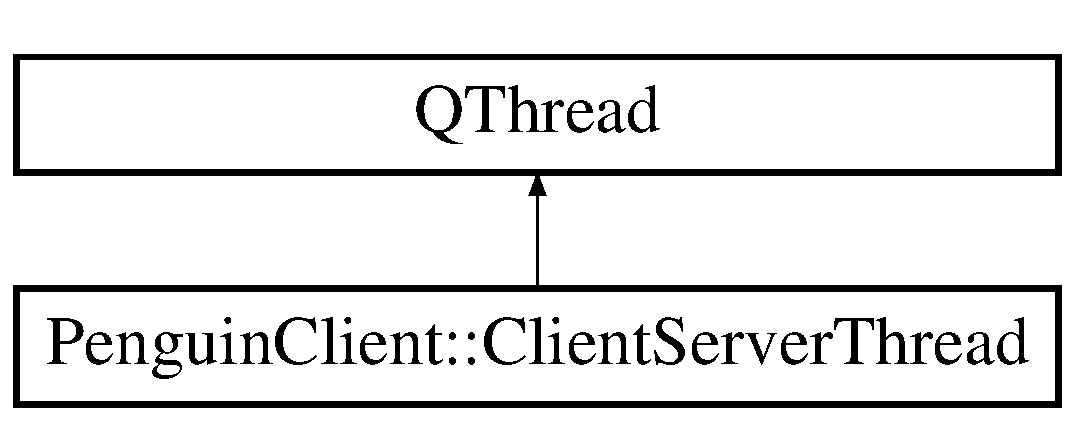
\includegraphics[height=2.000000cm]{classPenguinClient_1_1ClientServerThread}
\end{center}
\end{figure}
\subsection*{Public Slots}
\begin{DoxyCompactItemize}
\item 
void \hyperlink{classPenguinClient_1_1ClientServerThread_ac900a0f88575edac07b986919252124a}{send\-Message\-To\-Server} (Message\-Envelop \&data\-To\-Send)
\begin{DoxyCompactList}\small\item\em send\-Message\-To\-Server outcoming message to server \end{DoxyCompactList}\item 
\hypertarget{classPenguinClient_1_1ClientServerThread_adcb5c4f0a262e466c7112b6936bf1afa}{void \hyperlink{classPenguinClient_1_1ClientServerThread_adcb5c4f0a262e466c7112b6936bf1afa}{ready\-Read} ()}\label{classPenguinClient_1_1ClientServerThread_adcb5c4f0a262e466c7112b6936bf1afa}

\begin{DoxyCompactList}\small\item\em ready\-Read slot for inherited signal ready\-Read (from Tcp\-Socket), which wake thread on incomming message \end{DoxyCompactList}\item 
\hypertarget{classPenguinClient_1_1ClientServerThread_aa7ec5ef2fe7b46a75f6e36981ed0853f}{void \hyperlink{classPenguinClient_1_1ClientServerThread_aa7ec5ef2fe7b46a75f6e36981ed0853f}{disconnected} ()}\label{classPenguinClient_1_1ClientServerThread_aa7ec5ef2fe7b46a75f6e36981ed0853f}

\begin{DoxyCompactList}\small\item\em disconnected slot for inherited signal disconnected (from Tcp\-Socket), which wake thread on incomming message \end{DoxyCompactList}\end{DoxyCompactItemize}
\subsection*{Signals}
\begin{DoxyCompactItemize}
\item 
void \hyperlink{classPenguinClient_1_1ClientServerThread_a43213b711e120e2e84c82c8e35480c5f}{signal\-To\-Client} (Message\-Envelop \&readed\-Data)
\begin{DoxyCompactList}\small\item\em signal\-To\-Client send message to client, to show him data, not in use now \end{DoxyCompactList}\item 
void \hyperlink{classPenguinClient_1_1ClientServerThread_afe6e7353d83b7abaeed8a5cd3d6d308b}{client\-List} (const Q\-List$<$ Q\-String $>$ client\-List)
\begin{DoxyCompactList}\small\item\em client\-List sends list of clients to G\-U\-I thread \end{DoxyCompactList}\item 
void \hyperlink{classPenguinClient_1_1ClientServerThread_ad9243936519761c34857b7be3e13305d}{incomming\-Call} (const Q\-String name, const Q\-Host\-Address I\-P, const quint16 his\-Port, const quint16 my\-Port)
\begin{DoxyCompactList}\small\item\em incomming\-Call 1. part of initializitiaon of call \end{DoxyCompactList}\item 
void \hyperlink{classPenguinClient_1_1ClientServerThread_a82b4668ed1c995b0e6c82ef0e1970630}{success\-Response\-Call} (const Q\-String name, const Q\-Host\-Address I\-P, const quint16 his\-Port, const quint16 my\-Port)
\begin{DoxyCompactList}\small\item\em success\-Response\-Call 2. part of initializitiaon of call \end{DoxyCompactList}\item 
\hypertarget{classPenguinClient_1_1ClientServerThread_acb0bacb6fc830edb2ea2d7e1a33b7256}{void \hyperlink{classPenguinClient_1_1ClientServerThread_acb0bacb6fc830edb2ea2d7e1a33b7256}{end\-Of\-Call} ()}\label{classPenguinClient_1_1ClientServerThread_acb0bacb6fc830edb2ea2d7e1a33b7256}

\begin{DoxyCompactList}\small\item\em end\-Of\-Call signal of ending call from other side \end{DoxyCompactList}\item 
void \hyperlink{classPenguinClient_1_1ClientServerThread_a9946be2e2851f3e87a17fbaa6da55c4f}{error} (int socket\-Error, const Q\-String \&message)
\begin{DoxyCompactList}\small\item\em error \end{DoxyCompactList}\end{DoxyCompactItemize}
\subsection*{Public Member Functions}
\begin{DoxyCompactItemize}
\item 
\hypertarget{classPenguinClient_1_1ClientServerThread_a22658f01ef195ca0ca894cfeb503efab}{{\bfseries Client\-Server\-Thread} (Q\-Object $\ast$parent=0)}\label{classPenguinClient_1_1ClientServerThread_a22658f01ef195ca0ca894cfeb503efab}

\item 
\hypertarget{classPenguinClient_1_1ClientServerThread_a0150b6ece694bd17d0b336db842ad785}{void {\bfseries init\-Thread} (const Q\-String \&server\-I\-P\-Adress, quint16 server\-Listen\-Port, Q\-String login)}\label{classPenguinClient_1_1ClientServerThread_a0150b6ece694bd17d0b336db842ad785}

\item 
\hypertarget{classPenguinClient_1_1ClientServerThread_ac16c04f5113ec2ea901f4ee035ab02f2}{void {\bfseries run} ()}\label{classPenguinClient_1_1ClientServerThread_ac16c04f5113ec2ea901f4ee035ab02f2}

\end{DoxyCompactItemize}


\subsection{Member Function Documentation}
\hypertarget{classPenguinClient_1_1ClientServerThread_afe6e7353d83b7abaeed8a5cd3d6d308b}{\index{Penguin\-Client\-::\-Client\-Server\-Thread@{Penguin\-Client\-::\-Client\-Server\-Thread}!client\-List@{client\-List}}
\index{client\-List@{client\-List}!PenguinClient::ClientServerThread@{Penguin\-Client\-::\-Client\-Server\-Thread}}
\subsubsection[{client\-List}]{\setlength{\rightskip}{0pt plus 5cm}void Penguin\-Client\-::\-Client\-Server\-Thread\-::client\-List (
\begin{DoxyParamCaption}
\item[{const Q\-List$<$ Q\-String $>$}]{client\-List}
\end{DoxyParamCaption}
)\hspace{0.3cm}{\ttfamily [signal]}}}\label{classPenguinClient_1_1ClientServerThread_afe6e7353d83b7abaeed8a5cd3d6d308b}


client\-List sends list of clients to G\-U\-I thread 


\begin{DoxyParams}[1]{Parameters}
\mbox{\tt out}  & {\em client\-List} & list of logins \\
\hline
\end{DoxyParams}
\hypertarget{classPenguinClient_1_1ClientServerThread_a9946be2e2851f3e87a17fbaa6da55c4f}{\index{Penguin\-Client\-::\-Client\-Server\-Thread@{Penguin\-Client\-::\-Client\-Server\-Thread}!error@{error}}
\index{error@{error}!PenguinClient::ClientServerThread@{Penguin\-Client\-::\-Client\-Server\-Thread}}
\subsubsection[{error}]{\setlength{\rightskip}{0pt plus 5cm}void Penguin\-Client\-::\-Client\-Server\-Thread\-::error (
\begin{DoxyParamCaption}
\item[{int}]{socket\-Error, }
\item[{const Q\-String \&}]{message}
\end{DoxyParamCaption}
)\hspace{0.3cm}{\ttfamily [signal]}}}\label{classPenguinClient_1_1ClientServerThread_a9946be2e2851f3e87a17fbaa6da55c4f}


error 


\begin{DoxyParams}[1]{Parameters}
\mbox{\tt out}  & {\em socket\-Error} & \\
\hline
\mbox{\tt out}  & {\em message} & \\
\hline
\end{DoxyParams}
\hypertarget{classPenguinClient_1_1ClientServerThread_ad9243936519761c34857b7be3e13305d}{\index{Penguin\-Client\-::\-Client\-Server\-Thread@{Penguin\-Client\-::\-Client\-Server\-Thread}!incomming\-Call@{incomming\-Call}}
\index{incomming\-Call@{incomming\-Call}!PenguinClient::ClientServerThread@{Penguin\-Client\-::\-Client\-Server\-Thread}}
\subsubsection[{incomming\-Call}]{\setlength{\rightskip}{0pt plus 5cm}void Penguin\-Client\-::\-Client\-Server\-Thread\-::incomming\-Call (
\begin{DoxyParamCaption}
\item[{const Q\-String}]{name, }
\item[{const Q\-Host\-Address}]{I\-P, }
\item[{const quint16}]{his\-Port, }
\item[{const quint16}]{my\-Port}
\end{DoxyParamCaption}
)\hspace{0.3cm}{\ttfamily [signal]}}}\label{classPenguinClient_1_1ClientServerThread_ad9243936519761c34857b7be3e13305d}


incomming\-Call 1. part of initializitiaon of call 


\begin{DoxyParams}[1]{Parameters}
\mbox{\tt out}  & {\em name} & login of person, who calls us \\
\hline
\mbox{\tt out}  & {\em I\-P} & of person, who calls us \\
\hline
\mbox{\tt out}  & {\em his\-Port} & port of person, who calls us \\
\hline
\mbox{\tt out}  & {\em my\-Port} & port, which this client uses for communication with server \\
\hline
\end{DoxyParams}
\hypertarget{classPenguinClient_1_1ClientServerThread_ac900a0f88575edac07b986919252124a}{\index{Penguin\-Client\-::\-Client\-Server\-Thread@{Penguin\-Client\-::\-Client\-Server\-Thread}!send\-Message\-To\-Server@{send\-Message\-To\-Server}}
\index{send\-Message\-To\-Server@{send\-Message\-To\-Server}!PenguinClient::ClientServerThread@{Penguin\-Client\-::\-Client\-Server\-Thread}}
\subsubsection[{send\-Message\-To\-Server}]{\setlength{\rightskip}{0pt plus 5cm}void Penguin\-Client\-::\-Client\-Server\-Thread\-::send\-Message\-To\-Server (
\begin{DoxyParamCaption}
\item[{Message\-Envelop \&}]{data\-To\-Send}
\end{DoxyParamCaption}
)\hspace{0.3cm}{\ttfamily [slot]}}}\label{classPenguinClient_1_1ClientServerThread_ac900a0f88575edac07b986919252124a}


send\-Message\-To\-Server outcoming message to server 


\begin{DoxyParams}{Parameters}
{\em data\-To\-Send} & non encrypted message from G\-U\-I thread \\
\hline
\end{DoxyParams}
\hypertarget{classPenguinClient_1_1ClientServerThread_a43213b711e120e2e84c82c8e35480c5f}{\index{Penguin\-Client\-::\-Client\-Server\-Thread@{Penguin\-Client\-::\-Client\-Server\-Thread}!signal\-To\-Client@{signal\-To\-Client}}
\index{signal\-To\-Client@{signal\-To\-Client}!PenguinClient::ClientServerThread@{Penguin\-Client\-::\-Client\-Server\-Thread}}
\subsubsection[{signal\-To\-Client}]{\setlength{\rightskip}{0pt plus 5cm}void Penguin\-Client\-::\-Client\-Server\-Thread\-::signal\-To\-Client (
\begin{DoxyParamCaption}
\item[{Message\-Envelop \&}]{readed\-Data}
\end{DoxyParamCaption}
)\hspace{0.3cm}{\ttfamily [signal]}}}\label{classPenguinClient_1_1ClientServerThread_a43213b711e120e2e84c82c8e35480c5f}


signal\-To\-Client send message to client, to show him data, not in use now 


\begin{DoxyParams}[1]{Parameters}
\mbox{\tt out}  & {\em readed\-Data} & not parsed data from server \\
\hline
\end{DoxyParams}
\hypertarget{classPenguinClient_1_1ClientServerThread_a82b4668ed1c995b0e6c82ef0e1970630}{\index{Penguin\-Client\-::\-Client\-Server\-Thread@{Penguin\-Client\-::\-Client\-Server\-Thread}!success\-Response\-Call@{success\-Response\-Call}}
\index{success\-Response\-Call@{success\-Response\-Call}!PenguinClient::ClientServerThread@{Penguin\-Client\-::\-Client\-Server\-Thread}}
\subsubsection[{success\-Response\-Call}]{\setlength{\rightskip}{0pt plus 5cm}void Penguin\-Client\-::\-Client\-Server\-Thread\-::success\-Response\-Call (
\begin{DoxyParamCaption}
\item[{const Q\-String}]{name, }
\item[{const Q\-Host\-Address}]{I\-P, }
\item[{const quint16}]{his\-Port, }
\item[{const quint16}]{my\-Port}
\end{DoxyParamCaption}
)\hspace{0.3cm}{\ttfamily [signal]}}}\label{classPenguinClient_1_1ClientServerThread_a82b4668ed1c995b0e6c82ef0e1970630}


success\-Response\-Call 2. part of initializitiaon of call 


\begin{DoxyParams}[1]{Parameters}
\mbox{\tt out}  & {\em name} & login of person, who calls us \\
\hline
\mbox{\tt out}  & {\em I\-P} & of person, who calls us \\
\hline
\mbox{\tt out}  & {\em his\-Port} & port of person, who calls us \\
\hline
\mbox{\tt out}  & {\em my\-Port} & port, which this client uses for communication with server \\
\hline
\end{DoxyParams}


The documentation for this class was generated from the following files\-:\begin{DoxyCompactItemize}
\item 
clientserverthread.\-h\item 
clientserverthread.\-cpp\end{DoxyCompactItemize}

\hypertarget{classPenguinClient_1_1ListenServer}{\section{Penguin\-Client\-:\-:Listen\-Server Class Reference}
\label{classPenguinClient_1_1ListenServer}\index{Penguin\-Client\-::\-Listen\-Server@{Penguin\-Client\-::\-Listen\-Server}}
}


The \hyperlink{classPenguinClient_1_1ListenServer}{Listen\-Server} class T\-C\-P server opened for communication between clients $\ast$.  




{\ttfamily \#include $<$c2clistenthread.\-h$>$}

Inheritance diagram for Penguin\-Client\-:\-:Listen\-Server\-:\begin{figure}[H]
\begin{center}
\leavevmode
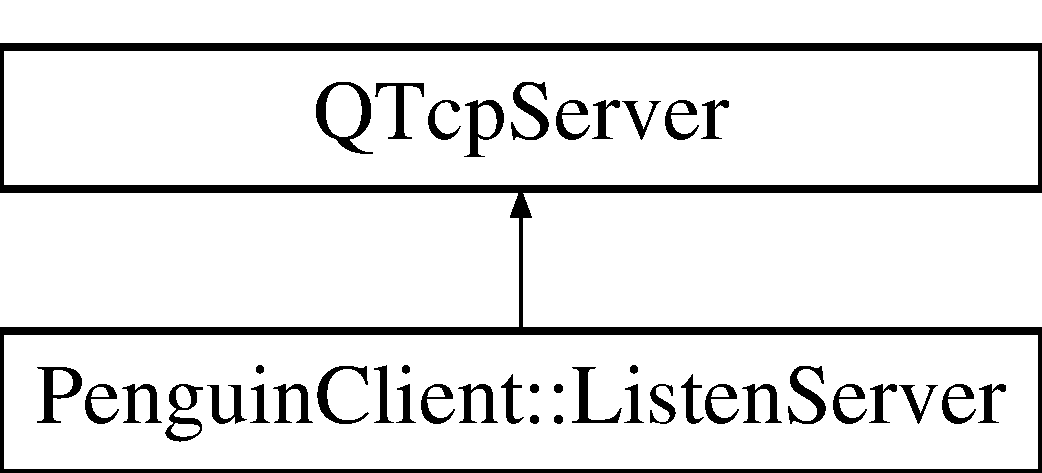
\includegraphics[height=2.000000cm]{classPenguinClient_1_1ListenServer}
\end{center}
\end{figure}
\subsection*{Signals}
\begin{DoxyCompactItemize}
\item 
\hypertarget{classPenguinClient_1_1ListenServer_ab74d4758471671d645b2b735f1e26991}{void {\bfseries end\-Connection} ()}\label{classPenguinClient_1_1ListenServer_ab74d4758471671d645b2b735f1e26991}

\end{DoxyCompactItemize}
\subsection*{Public Member Functions}
\begin{DoxyCompactItemize}
\item 
\hypertarget{classPenguinClient_1_1ListenServer_adb2d8a57702edd4efba425d0f3032795}{{\bfseries Listen\-Server} (Q\-Object $\ast$parent=0)}\label{classPenguinClient_1_1ListenServer_adb2d8a57702edd4efba425d0f3032795}

\item 
void \hyperlink{classPenguinClient_1_1ListenServer_aa122118cd9b60c0a1caea453d3fc2bec}{start\-Server} (const Q\-Host\-Address host\-Name, const quint16 port)
\begin{DoxyCompactList}\small\item\em start\-Server starts server on given host name and port \end{DoxyCompactList}\end{DoxyCompactItemize}
\subsection*{Protected Member Functions}
\begin{DoxyCompactItemize}
\item 
void \hyperlink{classPenguinClient_1_1ListenServer_ad31c26e1ca9ee83a753164643e7ab81d}{incoming\-Connection} (qintptr socket\-Descriptor)
\begin{DoxyCompactList}\small\item\em incoming\-Connection incoming connection management, starts new thread for incoming connection \end{DoxyCompactList}\end{DoxyCompactItemize}


\subsection{Detailed Description}
The \hyperlink{classPenguinClient_1_1ListenServer}{Listen\-Server} class T\-C\-P server opened for communication between clients $\ast$. 

\subsection{Member Function Documentation}
\hypertarget{classPenguinClient_1_1ListenServer_ad31c26e1ca9ee83a753164643e7ab81d}{\index{Penguin\-Client\-::\-Listen\-Server@{Penguin\-Client\-::\-Listen\-Server}!incoming\-Connection@{incoming\-Connection}}
\index{incoming\-Connection@{incoming\-Connection}!PenguinClient::ListenServer@{Penguin\-Client\-::\-Listen\-Server}}
\subsubsection[{incoming\-Connection}]{\setlength{\rightskip}{0pt plus 5cm}void Penguin\-Client\-::\-Listen\-Server\-::incoming\-Connection (
\begin{DoxyParamCaption}
\item[{qintptr}]{socket\-Descriptor}
\end{DoxyParamCaption}
)\hspace{0.3cm}{\ttfamily [protected]}}}\label{classPenguinClient_1_1ListenServer_ad31c26e1ca9ee83a753164643e7ab81d}


incoming\-Connection incoming connection management, starts new thread for incoming connection 


\begin{DoxyParams}{Parameters}
{\em socket\-Descriptor} & \\
\hline
\end{DoxyParams}
\hypertarget{classPenguinClient_1_1ListenServer_aa122118cd9b60c0a1caea453d3fc2bec}{\index{Penguin\-Client\-::\-Listen\-Server@{Penguin\-Client\-::\-Listen\-Server}!start\-Server@{start\-Server}}
\index{start\-Server@{start\-Server}!PenguinClient::ListenServer@{Penguin\-Client\-::\-Listen\-Server}}
\subsubsection[{start\-Server}]{\setlength{\rightskip}{0pt plus 5cm}void Penguin\-Client\-::\-Listen\-Server\-::start\-Server (
\begin{DoxyParamCaption}
\item[{const Q\-Host\-Address}]{host\-Name, }
\item[{const quint16}]{port}
\end{DoxyParamCaption}
)}}\label{classPenguinClient_1_1ListenServer_aa122118cd9b60c0a1caea453d3fc2bec}


start\-Server starts server on given host name and port 


\begin{DoxyParams}{Parameters}
{\em host\-Name} & \\
\hline
{\em port} & \\
\hline
\end{DoxyParams}


The documentation for this class was generated from the following files\-:\begin{DoxyCompactItemize}
\item 
c2clistenthread.\-h\item 
c2clistenthread.\-cpp\end{DoxyCompactItemize}

%--- End generated contents ---

% Index
\newpage
\phantomsection
\addcontentsline{toc}{part}{Index}
\printindex

\end{document}
